%Smart wheelchairs are wheelchairs with additional sensors and computers,
%enabling greater usability and safety. This can come in the form of alternative input methods,
%such as eye-gaze tracking \cite{eidNovelEyeGazeControlledWheelchair2016} or using a brain-computer
%interface \cite{kaufmannBraincomputerInterfaceBased2014} to control the wheelchair. For people with vision impairment,
%haptic feedback \cite{kondoNavigationGuidanceControl2008}\cite{vanderpoortenPoweredWheelchairNavigation2012}
%has been used to improve awareness of the surrounding environment and make indoor navigation safer.


\subsection{Sensors and hardware}
%To perceive the environment, the wheelchair should be fitted with various sensors and
%a compute element to process the sensors output.

\subsubsection{Sensor types}
Smart wheelchairs have used a varied range of sensor types to perceive the surrounding environment.
RGB-D stereo cameras have been widely used in the field \cite{wangS2P2SelfSupervisedGoalDirected2021}\cite{wangSelfSupervisedDrivableArea2019}\cite{jainAutomatedPerceptionSafe2014},
alongside 2D Lidar \cite{scudellariSelfdrivingWheelchairsDebut2017} and ultrasonic sensors \cite{levineNavChairAssistiveWheelchair1999}.
Self-driving cars built by companies such as Tesla and Waymo
use cameras, mmWave Radar, and 3D Lidar to avoid traffic and pedestrians \cite{karpathyTeslaAIDay2021}.

Selecting a sensor to use is not necessarily an either-or decision. Sensor fusion algorithms such as
the Extended Kalman Filter (EKF) or Unscented Kalman Filter (UKF) \cite{wanUnscentedKalmanFilter2000} allow
outputs from multiple sensors to be used together to improve their accuracy. Additionally, sensors can
be used for different applications on the smart wheelchair - a stereo camera could be used to sense the surrounding environment
while an inertial measurement unit (IMU) could be used for wheelchair odometry.
\Cref{table:sensor_options} compares several available sensor types,
taking into account factors such as resolution, cost, and accuracy.

\begin{table}[H]
    \centering
\begin{adjustbox}{width=\textwidth}
    \begin{tabular}{c c c}
    \toprule
    Sensor & Advantages & Disadvantages \\
    \midrule
    RGB-D Stereo Camera & Very high resolution & Low field of view (FOV) \\
    mmWave Radar & High accuracy & Low resolution \\
    3D Lidar & High resolution and accuracy & Very high cost \\
    2D Lidar & High FOV and accuracy & Only detects obstacles within the same plane \\
    Ultrasonic sensor & Low cost & One-dimensional \\
    \bottomrule
    \end{tabular}
\end{adjustbox}
    \caption{Sensor comparisons}
    \label{table:sensor_options}
\end{table}

% Description of different sensor types?

\subsubsection{RGB-D cameras}
One advantage RGB-D cameras have over alternative sensors is high RGB resolution,
allowing them to utilise advances in machine learning and computer vision.
Technologies such as Lidar may fail at path detection, as path markings
cannot be detected.

When comparing these cameras, factors such as package size,
field of view, and operating range are important to consider.
Several commercial options are compared in \Cref{table:stereo_camera}
- all of the listed units come with an integrated IMU.

\begin{landscape}
\begin{table}[H]
    \centering
    \begin{tabular}{c c c c c c}
    \toprule
    Name & Type & Cost (AUD)\footnotemark[1] & Dimensions (mm) \\
    \midrule
    Stereolabs Zed Mini \cite{stereolabsZEDMiniCamera2018} & Passive & \$595 & $124.5\times 30.5\times 26.5$ \\
    Stereolabs Zed 2 \cite{stereolabsZEDCameraSDK2019} & Passive & \$670 & $175\times 30\times 33$ \\
    Intel RealSense D455 \cite{intelIntelRealSenseProduct2022} & Active IR (Stereo) & \$595 & $124\times 26\times 29$ \\
    Microsoft Azure Kinect DK \cite{microsoftAzureKinectDK2021} & Active IR (Time of Flight)\footnotemark[2] & \$595 & $103\times 39\times 126$ \\
    \bottomrule
    \end{tabular}
    \caption{Stereo camera options}
    \label{table:stereo_camera}
\end{table}
\addtocounter{table}{-1}
\begin{table}[H]
    \centering
    \begin{tabular}{c c c c c c}
    \toprule
    Name & FOV (Horizontal, Vertical, Depth) & Operating Range (m) \\
    \midrule
    Stereolabs Zed Mini \cite{stereolabsZEDMiniCamera2018} & $90\degree\times 60\degree\times 100\degree$ & 0.1-15\\
    Stereolabs Zed 2 \cite{stereolabsZEDCameraSDK2019} & $110\degree\times 70\degree\times 120\degree$ & 0.3-20 \\
    Intel RealSense D455 \cite{intelIntelRealSenseProduct2022} & $90\degree\times 65\degree\times 87\degree$ & 0.6-6 \\
    Microsoft Azure Kinect DK \cite{microsoftAzureKinectDK2021} & $75\degree\times 65\degree\times 75\degree$ & 0.5-3.86 \\
    \bottomrule
    \end{tabular}
    \captionsetup{list=no}
    \caption{Stereo camera options (continued)}
\end{table}

\begin{table}[H]
    \centering
\begin{adjustbox}{width=1.25\textwidth}
    \begin{tabular}{c c c c c c}
    \toprule
    Name & Cost (AUD)\footnotemark[1] & Release Year & Speed & Power & Notes \\
    \midrule
    Nvidia Jetson Nano \cite{nvidiaJetsonNanoSystemonModule2019} & \$150 & Early 2019 & 0.5 TFLOPS (FP16) & 10 W & - \\
    Nvidia Jetson Xavier NX \cite{nvidiaJetsonXavierNX2019} & \$595 & Late 2019 & 21 TOPS (INT8) & 20 W & - \\
    Nvidia RTX 2080 \cite{nvidiaTuringGPUArchitecture2018} & \$1040 & 2018 & \makecell{80.5 TFLOPS (FP16)\\161.1 TOPS (INT8)} & 215 W & Doesn't include single-board computer \\
    Google Coral Edge TPU \cite{googlecoralCoralDevBoard2020} & \$190 & 2020 & 4 TOPS (INT8) & 2 W & Only supports TensorFlow Lite \\
    \bottomrule
    \end{tabular}
\end{adjustbox}
    \caption{AI accelerator options}
    \label{table:compute_element}
\end{table}
\end{landscape}

\footnotetext[1]{Costs are taken at RRP with an exchange rate of 1 AUD = 0.74 USD}
\footnotetext[2]{The Microsoft Azure Kinect DK has multiple operating modes that trade-off between FOV, operating range, and resolution. The \texttt{NFOV unbinned} mode was compared, which provides good trade-off between operating range and resolution.}

A caveat of the Stereolabs products is that they require a separate CUDA-enabled GPU (manufactured by Nvidia) to generate the point-cloud
and RGB-D image. In contrast, the Kinect DK only requires a CPU for processing, while the Intel RealSense performs processing onboard
and requires a USB-C 3.1 interface to communicate.

\subsubsection{Compute element}
A compute element inside a semi-autonomous driving system generally consists of several components -
a microcontroller to process user inputs and
send signals to the motors, a general-purpose computer to run pathfinding algorithms and log information,
and an AI accelerator to improve the performance of on-board machine learning (ML) algorithms.

AI accelerators use specialised hardware to perform operations common in ML algorithms (such as matrix multiplication
and convolution) more efficiently than a CPU can. GPUs have been used widely for this application; however, their high
power usage is infeasible for some applications. Embedded AI accelerators aim to provide greater power efficiency
at the cost of specialisation.

Machine learning models often use mixed-precision (FP16) datatypes to store weights while training.
Although improving the model's accuracy, FP16 datatypes are slow to manipulate during inference.
Model quantisation \cite{jacobQuantizationTrainingNeural2017} is a process where this FP16 datatype is replaced with an
INT8 datatype (using a scaling factor and bias) after training.
Quantisation greatly improves speed while only losing a small amount of model accuracy.
For this reason, modern AI accelerators focus on the performance of INT8 operations (TOPS, $10^9$ operations per second),
whereas earlier accelerators state the performance of FP16 operations (TFLOPS, $10^9$ floating-point
operations per second).

The Nvidia Jetson and Google Coral products are both popular options for embedded AI acceleration. These accelerators are compared
in \Cref{table:compute_element} alongside a gaming GPU. 

\pagebreak
\subsection{Scene understanding}
Scene understanding is a broad field and involves using computer vision methods
on visual or spatial data to gain better knowledge about the surrounding environment.
Convolutional Neural Networks (CNNs) are commonly used for this application, as they
can exploit the local nature of image features to reduce the number of required computations.

\subsubsection{Image classification}
Image classification is a core problem within this field and involves identifying the subject of an image (such as an animal or object).
AlexNet \cite{krizhevskyImageNetClassificationDeep2012}, based on the earlier digit-recognition CNN LeNet-5
\cite{lecunGradientbasedLearningApplied1998}, was one of the first deep CNNs
applied to this problem. AlexNet was trained on the large ImageNet dataset \cite{jiadengImageNetLargescaleHierarchical2009},
which consists of 15M images and 22K categories,
and achieved an error of only 15.3\% on a 1000 class subset. The underlying architecture uses a series of 5 convolutional
layers and 3 fully connected layers, which can be seen in \cref{fig:alexnet_architecture}.

\begin{figure}[b]
    \centering
    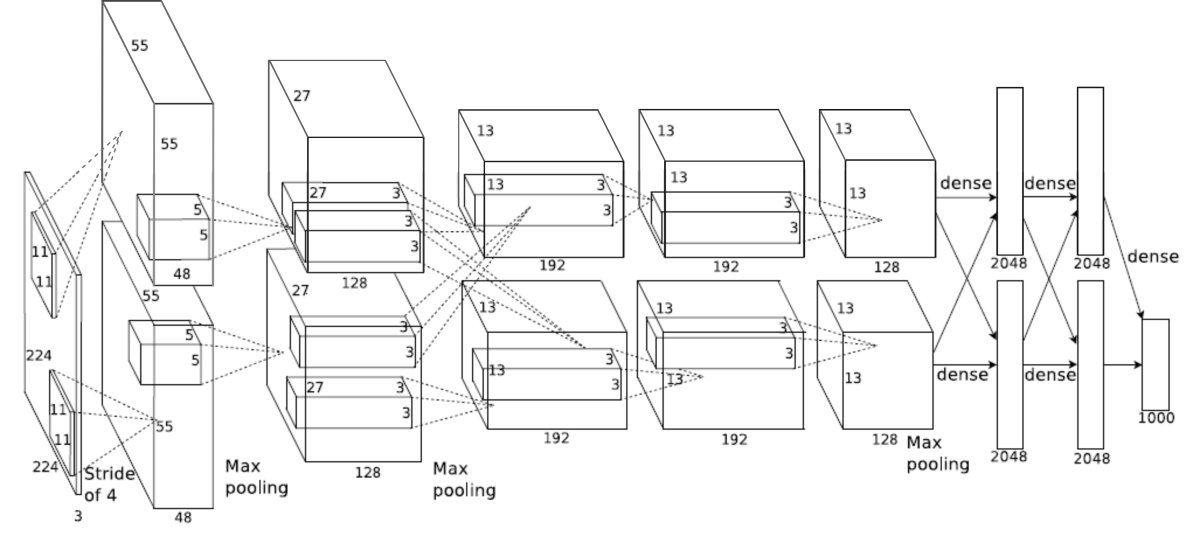
\includegraphics[width=0.8\linewidth]{images/alexnet_architecture.png}
    \caption{Architecture of the AlexNet image classification network. Reproduced from Krizhevsky et al. \cite{krizhevskyImageNetClassificationDeep2012}}
    \label{fig:alexnet_architecture}
\end{figure}

Neural network architectures have become deeper and more accurate over time, enabled by both
growth in computational power and dataset size. VGG-16 \cite{simonyanVeryDeepConvolutional2014}
and GoogLeNet \cite{szegedyGoingDeeperConvolutions2014}
are 16 and 22 layers deep respectively, and approached
human performance on the ImageNet dataset. ResNet \cite{heDeepResidualLearning2016} is up to 156 layers deep,
and exceeds human performance at image classification with an error of 3.57\%.
ResNet uses a 'skipping' architecture to improve network training, where the output of a layer relies directly on
the input of a previous layer.

\subsubsection{Object localisation}
Object localisation is another core problem within this field, and involves identifying the location of objects within an image as well as classifying them.
Object localisation can be used on a semi-autonomous wheelchair to identify
a pedestrian or obstacle within the environment. R-CNN \cite{girshickRichFeatureHierarchies2013} was one of the
first object classification models which utilised convolutional networks, by identifying potential bounding boxes
and running an image classifier on these bounding boxes. Fast and Faster R-CNN \cite{girshickFastRCNN2015}\cite{renFasterRCNNRealTime2015}
improved the speed of this model by running an image classifier backbone once on the entire image, and using a CNN to improve
the identification of bounding boxes. Pascal VOC \cite{everinghamPascalVisualObject2009} and MS COCO \cite{linMicrosoftCOCOCommon2014}
are datasets that are commonly used to evaluate object classification models.

YOLO (You Only Look Once) \cite{redmonYouOnlyLook2015}\cite{redmonYOLO9000BetterFaster2016}\cite{redmonYOLOv3IncrementalImprovement2018}\cite{bochkovskiyYOLOv4OptimalSpeed2020}
is another object classification model which focuses on improving the speed of the model. In particular, YOLOv4 \cite{bochkovskiyYOLOv4OptimalSpeed2020}
reaches over 60 fps (frames per second) on the Tesla V100, which enables its use in real-time applications such as autonomous driving and security camera footage. % RCNN and YOLO
YOLO divides an image into an $S\times S$ grid, and uses a single convolutional network to output both bounding box predictions and
an image classification for each grid square. Low probability and overlapping bounding boxes are then removed before the final output.
%YOLOv4 uses a backbone-neck-head architecture

\subsubsection{Semantic segmentation}
Semantic segmentation involves labelling each pixel of an object, rather than drawing a bounding box around the entire object.
This technique is often used in medical applications, where different components of a scan need to be labelled.
Another application semantic segmentation can be used for is drivable area detection, as a bounding box would not be able to cleanly
identify a road or kerb. \Cref{fig:classification_types} compares the output of semantic segmentation to image classification and object localisation.

Most semantic segmentation algorithms use an encoder-decoder architecture, where information about the image is encoded into a small feature space.
This feature space is then decoded back to the size of the original image using deconvolutional layers to obtain the segmented output.
Encoding is typically done using a pre-trained model backbone, such as ResNet, which reduces the computational power required to train
the model.
An issue with this architecture is that the resulting segmentation can be low quality, as the image encoding is low resolution.
U-net \cite{ronnebergerUNetConvolutionalNetworks2015} is a semantic segmentation network that helps to rectify this issue,
by using higher-resolution features during deconvolution.
This makes the segmented output sharper and more accurate.

Another semantic segmentation algorithm is DeepLab \cite{chenSemanticImageSegmentation2014}\cite{chenDeepLabSemanticImage2016}\cite{chenRethinkingAtrousConvolution2017}.
DeepLab uses atrous convolution (otherwise known as dilated convolution), which is a type of convolution that widens the FOV of a convolutional layer.
It does this by leaving gaps in the convolutional layer, as illustrated in \cref{fig:atrous_convolution}.
By widening the FOV of each convolution, less downscaling is required during encoding. This allows the image to be encoded in a much higher resolution,
leading to a more accurate output.
To obtain the segmented output, a technique called atrous spatial pyramid pooling (ASPP) is used. ASPP samples the feature space at different
scales using atrous convolution to classify each pixel in the image.
These techniques improve both the accuracy and speed of the network - DeepLabv3 obtained 86.9\% accuracy on the PASCAL VOC 2012 test set.

\begin{figure}[h]
    \centering
    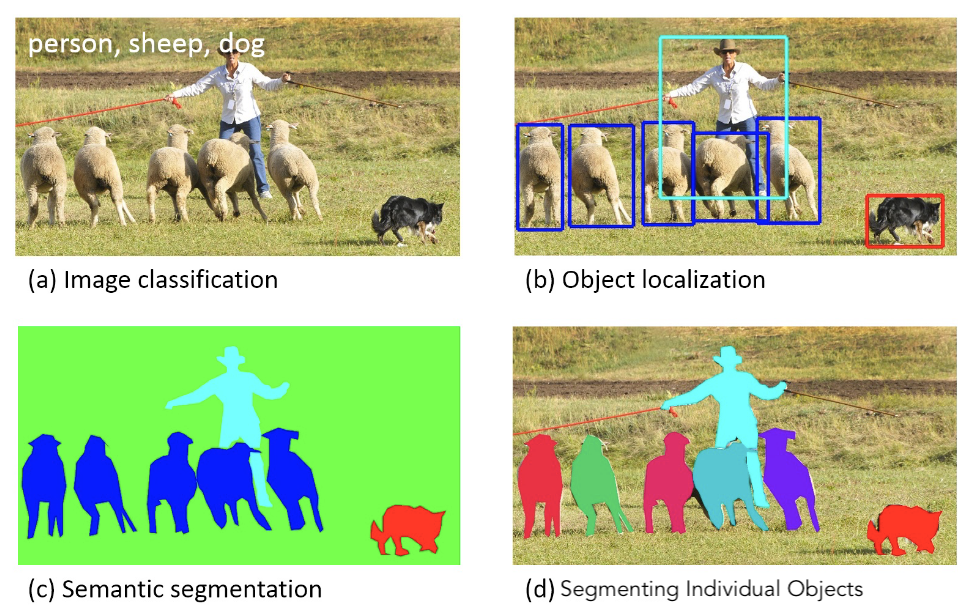
\includegraphics[width=0.6\linewidth]{images/classification_types.png}
    \caption{Types of classification in machine vision. Reproduced from Lin et al. \cite{linMicrosoftCOCOCommon2014}}
    \label{fig:classification_types}
\end{figure}

\begin{figure}[b]
    \centering
    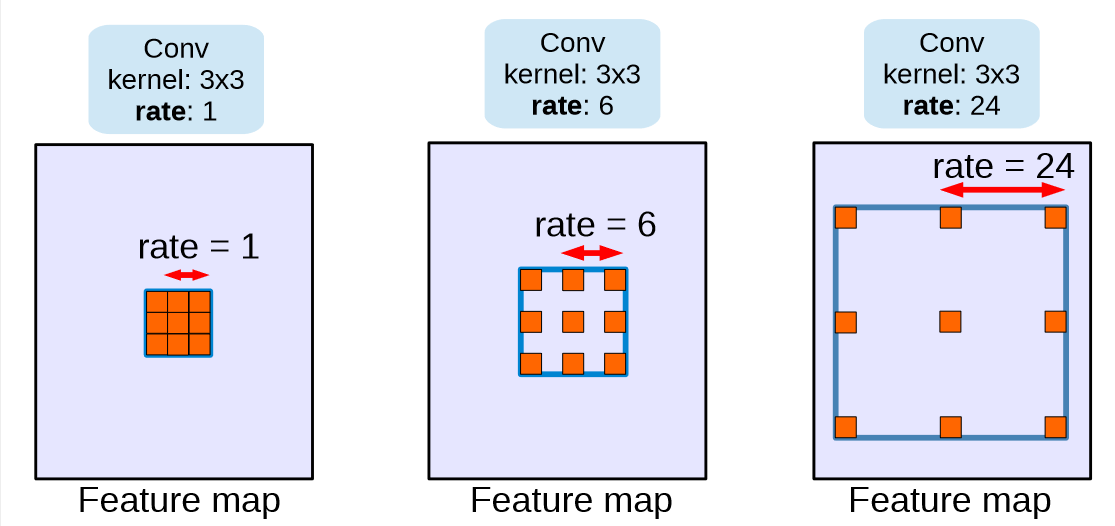
\includegraphics[width=0.6\linewidth]{images/atrous_convolution.png}
    \caption{Atrous convolution with a 3x3 kernel, showing increasing FOV. Reproduced from Chen et al. \cite{chenRethinkingAtrousConvolution2017}}
    \label{fig:atrous_convolution}
\end{figure}

\pagebreak
\subsubsection{Autonomous driving}
Autonomous driving and autonomous wheelchair control involve similar challenges,
including drivable area segmentation and object detection. As described previously, many machine learning
models utilise an image classification backbone to extract features from an image, with a `detection head'
then used for the final prediction.

Running multiple classification backbones for different models can be inefficient, as
the work of feature extraction is duplicated many times over. One way to improve the performance
of the autonomous system is to share a classification backbone between models, and use different detection
heads for various tasks.

An example of this architecture is HydraNets \cite{karpathyTeslaAIDay2021}, a machine learning model used by
Tesla to perform tasks such as traffic light detection, lane prediction, and object detection efficiently.
Other machine learning models that utilise this architecture include YOLOP \cite{wuYOLOPYouOnly2021} and
Hybridnet \cite{vuHybridNetsEndtoEndPerception2022}, which focus on lane segmentation, drivable area segmentation,
and object detection. The model architecture of YOLOP is shown in \cref{fig:yolop}.

This approach is valuable in situations where compute hardware is limited. Real-time applications such as
autonomous wheelchair control require fast inference times to react to obstacles in the surrounding environment.

\begin{figure}[b]
    \centering
    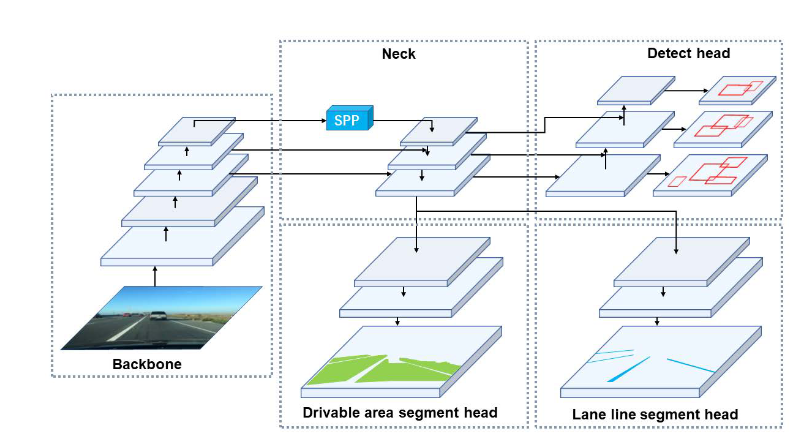
\includegraphics[width=0.65\linewidth]{images/yolop.png}
    \caption{YOLOP model architecture. Reproduced from Wu et al. \cite{wuYOLOPYouOnly2021}}
    \label{fig:yolop}
\end{figure}

To train these ML models, a pre-trained model backbone (on a dataset such as ImageNet \cite{jiadengImageNetLargescaleHierarchical2009})
is retrained on a driving dataset. This technique is known as transfer learning, and can vastly reduce the amount of time required
to train a new model.
Driving datasets such as Cityscapes \cite{cordtsCityscapesDatasetSemantic2016} and Berkeley DeepDrive \cite{yuBDD100KDiverseDriving2018}
can be used for this purpose. Additionally, game-engine based driving simulators such as CARLA \cite{dosovitskiyCARLAOpenUrban2017} can be used to generate a
synthetic dataset for training.

% U-net, deepnet

% classification, localization, segmentation, video, datasets
% SLAM, mapping, hybridnet, etc.
% Transfer Learning & Datasets

\pagebreak
\subsection{Assistive control}
Once an understanding of the 3D scene has been built, the user can be navigated through the environment.
The surrounding environment is generally represented as an occupancy grid \cite{elfesUsingOccupancyGrids1989},
which is a top-down view of the area where each grid cell indicates the probability that it is occupied
by an obstacle. It is possible to include more detailed information about
paths and obstacles by adding more information to the occupancy grid.

In semi-autonomous control, the user decides the desired speed and direction of the wheelchair, with any intervention only
occurring before a collision takes place. This is in contrast to full autonomy, where the user specifies the
desired end goal and the wheelchair navigates to that goal \cite{wangS2P2SelfSupervisedGoalDirected2021}.
%In full autonomous control, SLAM is required to build a global map of the surroundings - this is not necessary
%for semi-autonomous control, as only a local map is needed for navigation assistance.

\subsubsection{Path-based algorithms}
Path-based algorithms take an occupancy grid as an input and output a path between the start point and a goal point.
A* is an example of this and uses a heuristic to efficiently find the shortest path between the start and end point.
Other algorithms such as RRT* (rapidly-exploring random tree) \cite{karamanSamplingbasedAlgorithmsOptimal2011} build a tree from randomly sampled points
to find a path to the goal node. RRT* may not find the shortest path initially, but can find an efficient path with much less
computation required.

\begin{figure}[b]
    \centering
    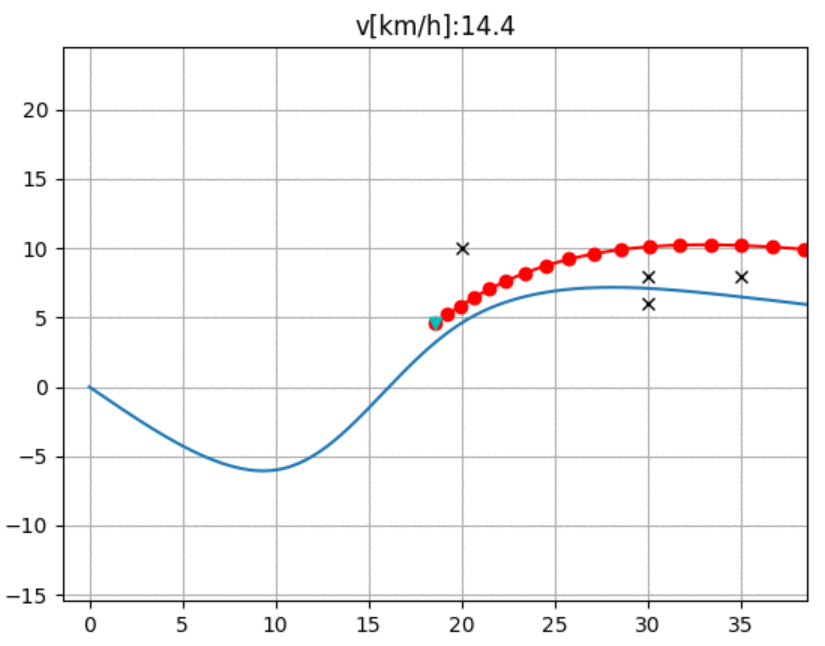
\includegraphics[width=0.5\linewidth]{images/frenet_frame_local_path.png}
    \caption{Fren\'et-Frame path planning, with reference path and local path illustrated. Reproduced from Sakai et al. \cite{sakaiPythonRoboticsPythonCode2018}}
    \label{fig:frenet_frame_local_path}
\end{figure}

One potential issue with these two algorithms is that they fail to take into account the smoothness of the resulting path.
Although the path may be short, sharp changes in the trajectory could be uncomfortable for the user.

Trajectory planning algorithms aim to solve this - one such algorithm is optimal-control in a Fren\'et-Frame \cite{werlingOptimalTrajectoryGeneration2010},
which can be used in autonomous vehicle control.
This algorithm takes a reference path as an input and outputs a local path that avoids collisions and minimises jerk (rate of change of acceleration).
This is done by generating sample trajectories (represented with quintic polynomials), removing those which cause collisions, and choosing
the remaining trajectory with the lowest change in acceleration. \Cref{fig:frenet_frame_local_path} illustrates the reference path, obstacles, and generated
local path in an example scenario.
It should be noted that this algorithm still requires a reference path, which could be generated
with one of the pathfinding algorithms mentioned above.

\subsubsection{Local algorithms}
Local algorithms only consider obstacles currently in the proximity of the wheelchair,
and use this information to set the current speed and direction of the wheelchair.
VFH+ (vector field histogram) \cite{ulrichVFHReliableObstacle1998} is one example, which
has been applied to wheelchair control algorithms in prior work \cite{tomariEnhancingWheelchairControl2014}.
VFH+ calculates a polar obstacle density histogram around the robot based on the occupancy grid.
The histogram is then binarized, to classify sectors around the robot as either occupied or not occupied.
Next, a masked polar histogram is generated, which excludes paths that are not possible given the robots
turning radius and kinematics. Finally, a safe direction is chosen which is nearest to the user's desired direction.
An example binary histogram is shown in \cref{fig:binary_histogram_vfh}; the chosen direction avoids the obstacle in the
desired direction.

\begin{figure}[b]
    \centering
    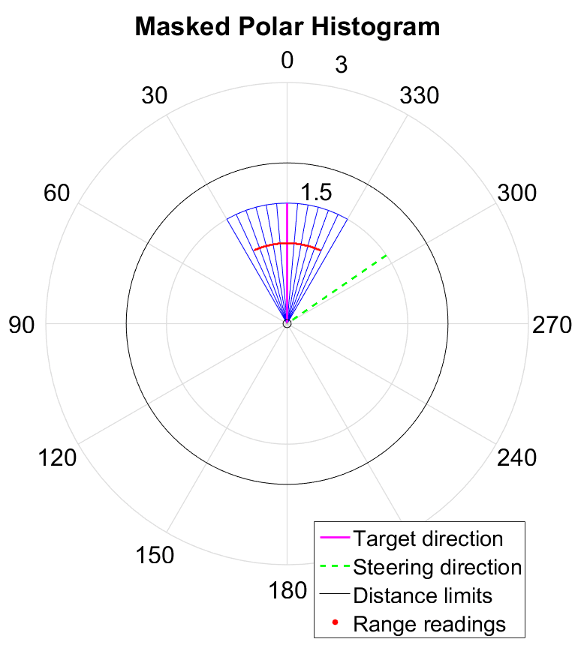
\includegraphics[width=0.38\linewidth]{images/binary_histogram_vfh.png}
    \caption{VFH+ binary histogram, representing the direction of obstacles. Reproduced from MathWorks \cite{mathworksVectorFieldHistogram2022}}
    \label{fig:binary_histogram_vfh}
\end{figure}
\pagebreak
An advantage to this algorithm is that it gives the user more fine-grained control over their speed and direction,
rather than planning a path to their assumed goal.
However an issue with VFH+ is that it does not control the wheelchair's speed, and instead only finds a safe direction.
Ideally, the wheelchair should slow down if an obstacle is present.

Another approach to assistive control with local algorithms is haptic feedback. Rather than
blending inputs from the autonomous software and the user, the joystick itself is actuated
to make it more difficult to move in the direction of obstacles \cite{kondoNavigationGuidanceControl2008}\cite{vanderpoortenPoweredWheelchairNavigation2012}.
An advantage of this approach is that it gives the user total control over which direction of movement they choose,
however, the additional force required to actuate the joystick may fatigue the user.

%\subsubsection{Path and Trajectory Planning}
%Path planning involves finding a path from the current location to the goal location.

%\subsubsection{Feedback and Control Blending}
%Alternative methods which can be used to provide assistance to the user are haptic feedback and control blending.


% Inputs
% Semi-autonomy
% Full autonomy
% Path Planning
% Obstacle avoidance
% 3D - 2D mapping

% Indoor vs Outdoor assistance.
% Sensors
% Machine Learning
%\cite{tomariEnhancingWheelchairControl2014}
